





\section{GRChombo}

\subsection{Numerical Discretisation of Spacetime}

euler step not stable, in comes runge kutta, mention there are other schemes but we don't use it

\subsubsection{Runge-Kutta Integration}

\subsubsection{Method of Lines}

\subsection{Boundary Conditions}

WRITE ABOUT A FEW LIEK REFLECTIVE ADN SOMMERFELD, FIND REF 1 IN MY Q PPAER FOR SOMMERFLED

\subsection{Overview of GRChombo}


WRITE MY OWN VERSION OF JOSS PAPER


GRChombo [] is a recently developed Numerical Relativity code built on top of Chombo [], a PDE solver with fully adaptive mesh refinement (AMR). The advantage of AMR is that regridding, and subsequently sub-volumes of high resolution, is calculated during runtime. This is especially useful for simulating fluids in GR as they can develop features requiring higher resolution in places a human may not expect making pre-specified mesh refinement hard to use. GRChombo uses the CCZ4 system with 1+log slicing and the Gamma driver shift condition, discussed in sections (). GRChombo also supports vectorisation and parallelisation with OpenMP and MPI making it suitable for use on supercomputer clusters. 

So far I have implemented initial data for a single or binary system of compact objects which can be either a Schwarzschild black hole or a boson star. The initial data uses isotropic coordinates and can be boosted along coordinate axes, but not yet general directions, giving the possibility of single boosted objects, accelerated head on collisions, grazing collisions and inspirals/quasi-orbits. It should be noted that my implementation was built on top of the pre-existing complex scalar field class (written by Miren). The remainder of this section will cover the numerical aspects of my work.

TALK MORE ABOUT GRCHOMBO AND MAYBE REF THE NEW PAPER


\subsection{Simulation Units}
MAKE THIS WORK WITH THE CONVENTIONS SECTION ASND THEN DESCRIBE WHAT IS NEW FOR ONLY THE SIMULATIONS

GRChombo defaults to geometric units, as described in section (1.2). The scalar field $\vp$ appears in the action as
\begin{equation} S = \int_{\M} \left[g^{\mu\nu}\partial_\mu \vp \partial_\nu \vp^* + ... \right]\dd x^4\end{equation}
and given $S$ and the metric are dimensionless, dimensional analysis tells us $\vp$ has units of inverse length in natural units, or units of energy. The Klein-Gordon mass $m$
\begin{equation} \Box \vp = m^2 \vp\end{equation}
can be absorbed into new dimensionless spatial coordinates $\tilde{x}^i = x^i m$ changing the KG equation to the scale invariant form.
\begin{equation} \Box \vp = \vp\end{equation}




\subsection{Boson Star Initial Data}

Following on from the EKG ODE's in Eqs.~(\ref{boson:eq:EKGODE1}),  (\ref{boson:eq:EKGODE2}) and (\ref{boson:eq:EKGODE3}) we now seek to solve them numerically to obtain initial data for a single static boson star. The system can be reduced to a set of five first order ODE's with five boundary conditions. For a physical star we would like to impose $\Phi(0) = \Phi_c$, $\Phi'(0)=0$, $\Phi(r\rightarrow\infty)\rightarrow0$, $\Omega'(0)=0$, $\Omega(r\rightarrow\infty)\rightarrow1$, $\Psi'(0)=0$ and $\Psi(r\rightarrow\infty)\rightarrow1$ to be regular at the origin and match the Schwarzschild vacuum solution at large radius; however this is seven boundary conditions and we can only impose five. The condition $\Omega(0)'=0$ cannot be specified as Eq.~(\ref{boson:eq:EKGODE1}) is first order in derivatives of $\Omega$ but given that $r$ and $\Psi'$ both vanish at the origin then $\Omega'$ must also vanish at the origin automatically. One more boundary condition can be removed by asking for the boson star solution to match the isotropic Schwarzschild solution in Eq.~(\ref{intro:eq:iso_bh}) and therefore,
\begin{equation}
\Omega = \left(\frac{1-\frac{m}{2r}}{1+\frac{m}{2r}}\right) \quad \& \quad \Psi = \left( 1+\frac{m}{2r}\right)^2 \end{equation} 
where $m$ can be interpreted as the mass of the boson star; this mass will not enter the boundary condition so can be safely ignored. Combining the two equations above gives
\begin{equation} 
\sqrt{\Psi}\left(1+\Omega\right) = 2
\end{equation}
for a vacuum spacetime. Imposing the single condition $\sqrt{\Psi(\infty)}\left(1+\Omega(\infty)\right)=2$, rather than both $\Omega(\infty)=1$ and $=\Psi(\infty)=1$, then gives asymptotic flatness in just one boundary condition. One final point of importance is the frequency $\omega$ turns the Klein-Gordon ODE into an eigenvalue problem, admitting only discrete values of $\omega$. 

The problem has now been reduced to five ODE's with the following five boundary conditions,
\begin{equation} \{\Phi(0),\Phi'(0),\Psi'(0),\Omega(0),\sqrt{\Psi(\infty)}\left(1+\Omega(\infty)\right);\omega \} = \{ \Phi_c,0,0,\omega_0,2;\omega_0\},\end{equation}
subjected to the condition of an eigenvalue $\omega=\omega_0$. The first attempt to find the radial profile $\{\Phi(r), \Omega(r), \Psi(r)\}$ of the boson star was to use a relaxation 
method [REF] as it trivially incorporates the above two-point boundary conditions. In practice this method did not work well with the eigenvalue problem in $\omega$.
Unlike with a shooting method, there was no obvious way of telling whether the guess $\omega$ was larger or
smaller than the correct value. Even if this problem were overcome, a numerical solution with relaxation is computationally slow, even with Successive Over-Relaxation [REF] [20]; perhaps a multigrid method could work here but a simpler method was used.


\subsubsection{Shooting Method}

To find the initial data for a single Boson star, a private {c++} script was written using RK4 [REF] to integrate the EKG system taking five initial conditions, and eigenvalue guess $\omega_0$, 
\begin{equation} \{\Phi(0),\Phi'(0),\Psi(0),\Psi'(0),\Omega(0);\omega \} = \{ \Phi_c,0,\Psi_c,0,\omega_0;\omega_0\}.\end{equation}
Unfortunately $\omega_0$ and $\Psi_c$ are unknown apriori, but guessing any values reasonably close to untity, such as $\omega_0=0.5$ and $\Psi_c=2$, still give a boson star. This will generally result in the following asymptotic metric,
\begin{equation} g_{\mu\nu}(r\rightarrow\infty) \rightarrow \mathrm{diag}(-A^2,B^2,B^2,B^2), \label{grchombo:eq:ABBB}\end{equation}
 for constant $A$ and $B$. 

 Before we discuss how to find the correct value of $\omega$, there is a subtle numerical problem to adress. Using spherical polar coordinates in flat space, the Klein-Gordon equation (\ref{boson:eq:KGeqn}) with $V=m^2 |\vp|^2$ and ansatz $\vp =\Phi_{flat}(r)e^{\mathrm{i}\omega t}$ reduces to,
\begin{align}
\frac{1}{\sqrt{-g}} \partial_\mu \left(\sqrt{-g} g^{\mu\nu} \partial_\nu \right)\vp &= \frac{\partial V}{\partial |\vp|^2} \vp ,\\
 \partial_t \left( g^{tt} \partial_t \right)\Phi_{flat}(r)e^{\mathrm{i} \omega t} + \frac{1}{r^2} \partial_r \left(r^2 g^{rr} \partial_r \right)\Phi_{flat}(r)e^{\mathrm{i} \omega t} &= m^2 \Phi_{flat}(r)e^{\mathrm{i} \omega t} ,\\
  \omega^2 \Phi_{flat}(r) + \frac{1}{r^2} \partial_r \left(r^2  \partial_r \right)\Phi_{flat}(r) &= m^2 \Phi_{flat}(r) ,\\
\end{align}
where $\sqrt{-g} = r^2 \sin(\theta)$, $g^{tt}=-1$ and $g^{rr}=1$. This has general solution,
\begin{equation}
\Phi_{flat}(r) = \frac{1}{r}\left(C_1 e^{- r \sqrt{m^2-\omega^2}} + C_2 e^{ r \sqrt{m^2-\omega^2}} \right),
\end{equation}
for $\Phi_{flat}(r)$ and two constants $C_1$ and $C_2$. Due to finite resolution during numerical integration, at large radius $C_2$ will never be exactly zero and will eventually grow (along increasing radius) and spoil the numerical integration; even though this behavour was derived in flat space it is still present in curved space with spherical symmetry - especially at such large radius that space is approximately flat. In practice, the scalar field $\Phi$ will decay to some value roughly twenty orders of magnitude smaller than the central density $\Phi(0)$ and is effectively zero within numerical noise. At this point the coefficient $C_2$ is excited by noise and starts to grow exponentially. At a radius $r_*$ when the growing mode is deemed to be dominating, usually detected by an axis crossing $(\Phi(r_*)=0$ or a turning point $\Phi'(r_*)=0)$ the conditions $\Phi(r>r_*)=\Phi'(r>r_*)=0$ are enforced during integration. This creates a vacuum for $r>r_*$ and the spacetime is pure Schwarzschild. After this point, an exponentially growing stepsize was used to reach radii of order $10^8$ to $10^{10}$ times larger than desired for evolutions and the values $A = \Omega_\infty= \sqrt{-g_{00}}$ and $B=\Psi_{\infty}=\sqrt{g_{ii}}$ can be read off.

Interval bisection was used to find the best value of $\omega$, $\omega_0$, to machine precision; for the ground state we can tell that $\omega>\omega_0$ if $\Phi(r)$ develops a turning point before an axis crossing and $\omega < \omega_0$ if $\Phi(r)$ develops an axis crossing before a turning point. To find the $n$'th excited state, which has $n$ axis crossing for $\Phi(r)$ and $\Phi(r\rightarrow \infty) \rightarrow 0$ a similar scheme is followed to find the eigenvalue $\omega_n$. If $\Phi(r)$ has $n+1$ axis crossings then $\omega>\omega_n$ and if $\Phi(r)$ has $n$ axis crossings followed by a turning point then $\omega<\omega_n$. This method of doing a numerical integration and iteratively restarting to get closer to the target solution is known as a shooting method.

Putting everything together, a boson star solution with eigen value $\omega_0$ (or $\omega_n$ for excited stars) and asymptotic metric Eq.~(\ref{grchombo:eq:ABBB}) can be obtained. To find a star with asymptotic metric $\eta_{\mu\nu}$ of flat space, the initial conditions are iteratively improved like $\Omega_c \rightarrow \Omega_c / \Omega_\infty$ and $\Psi_c \rightarrow \Psi_c / \Psi_\infty$; the interval bisection for $\omega$ is then restarted. This is iterated three to five times which leaves $A=\Omega_\infty=1$ and $B=\Psi_\infty=1$ to extreme precision and the isotropic boson star is created. This whole process requires a few seconds runtime for a high resolution 200,000 grid-point simulation on a regular laptop.




%   \begin{figure}[h!]
%   \caption{Boson Star radial profile, Left: Ground state, Right: 1st Excited state}
%   \centering
%   \subfloat{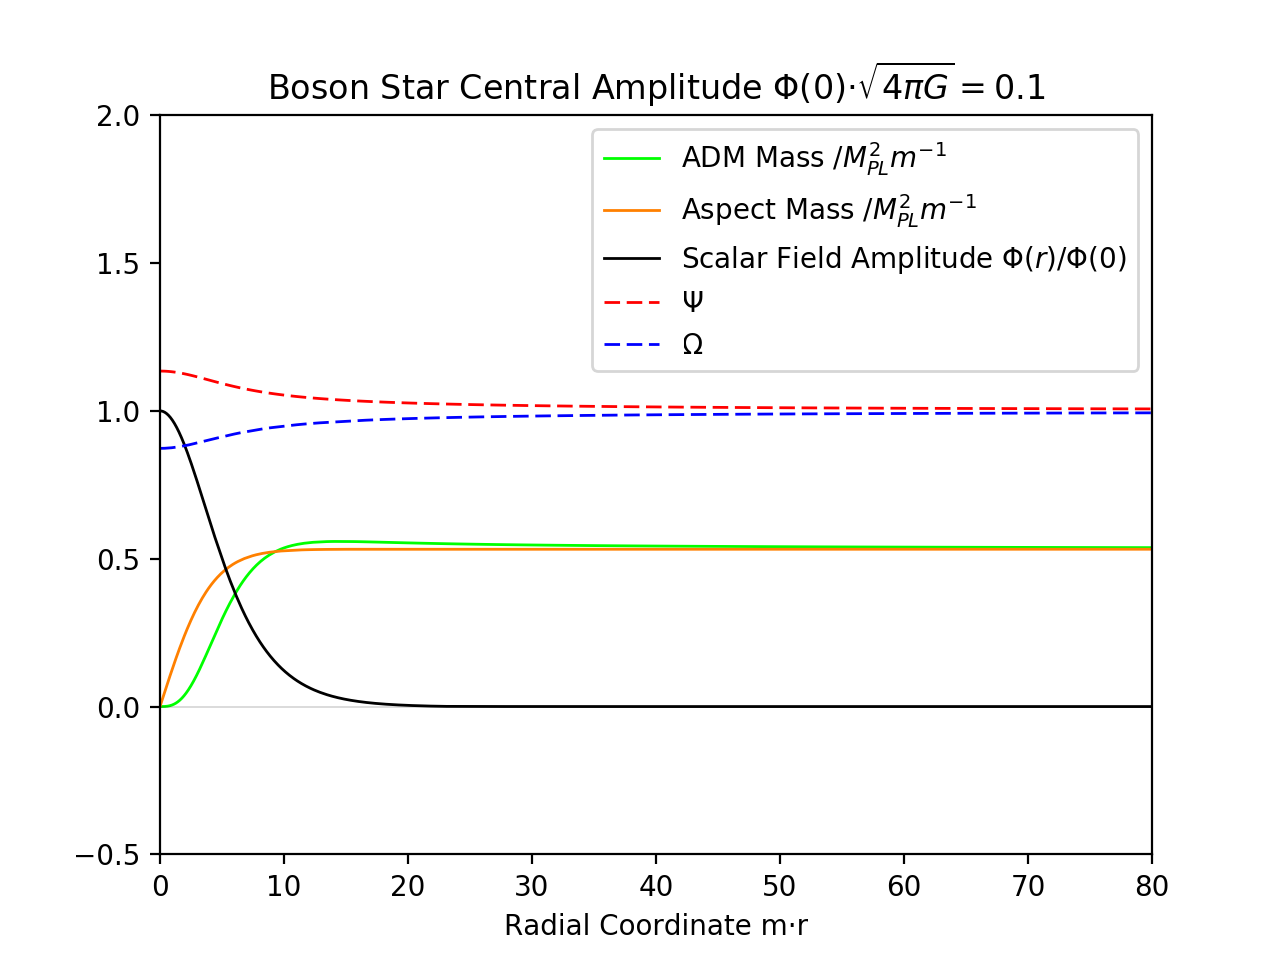
\includegraphics[width=0.5\textwidth]{png/bosonstar_groundstate.png}\label{boson:fig:f1}}
%   \hfill
%   \subfloat{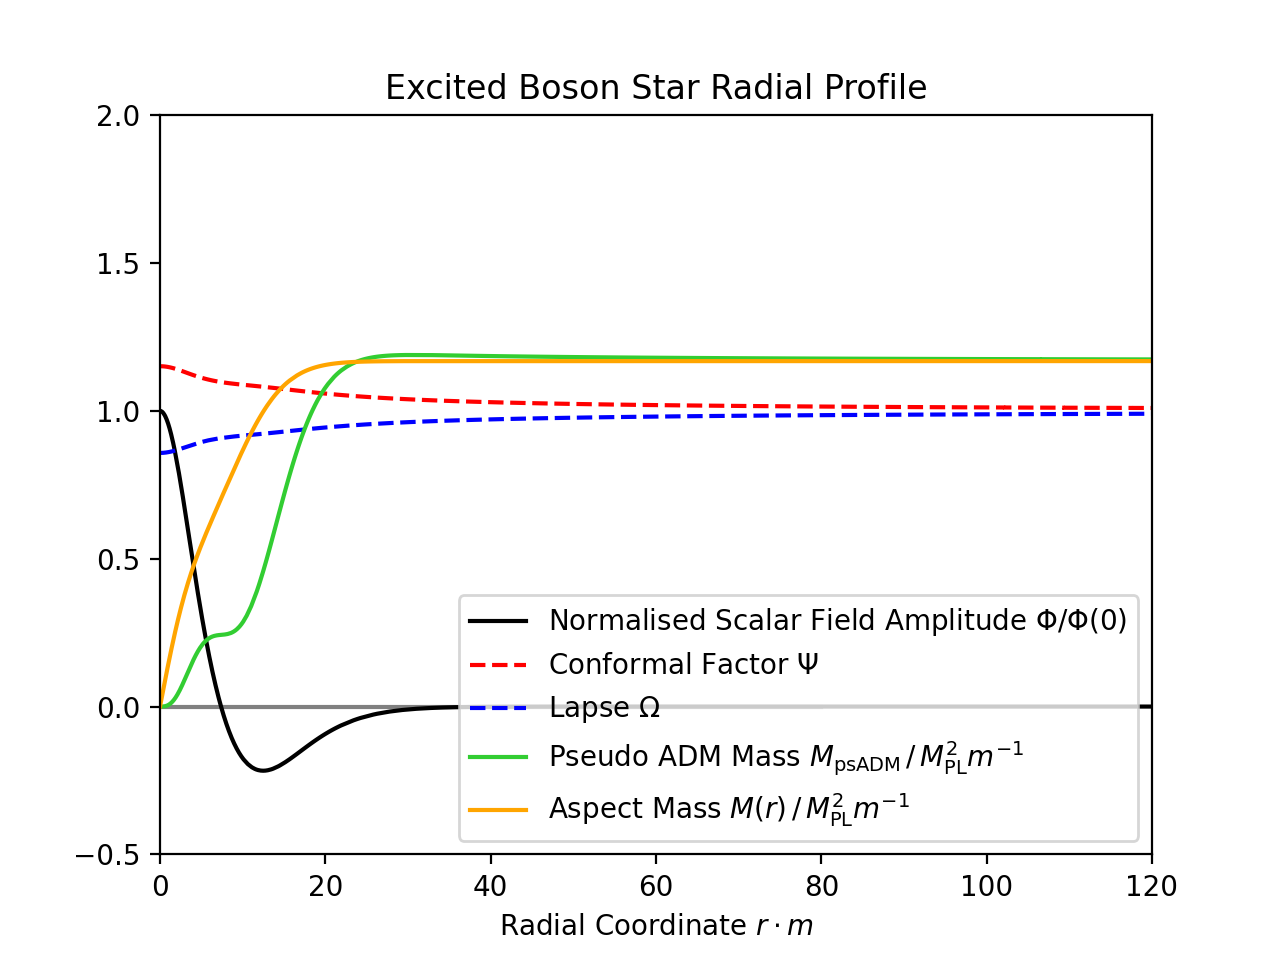
\includegraphics[width=0.5\textwidth]{png/bosonstar_excitedstate.png}\label{boson:fig:f2}}
% \end{figure}

  \begin{figure}[h!]
  \caption{Boson star radial profile for the ground state}
  \centering
  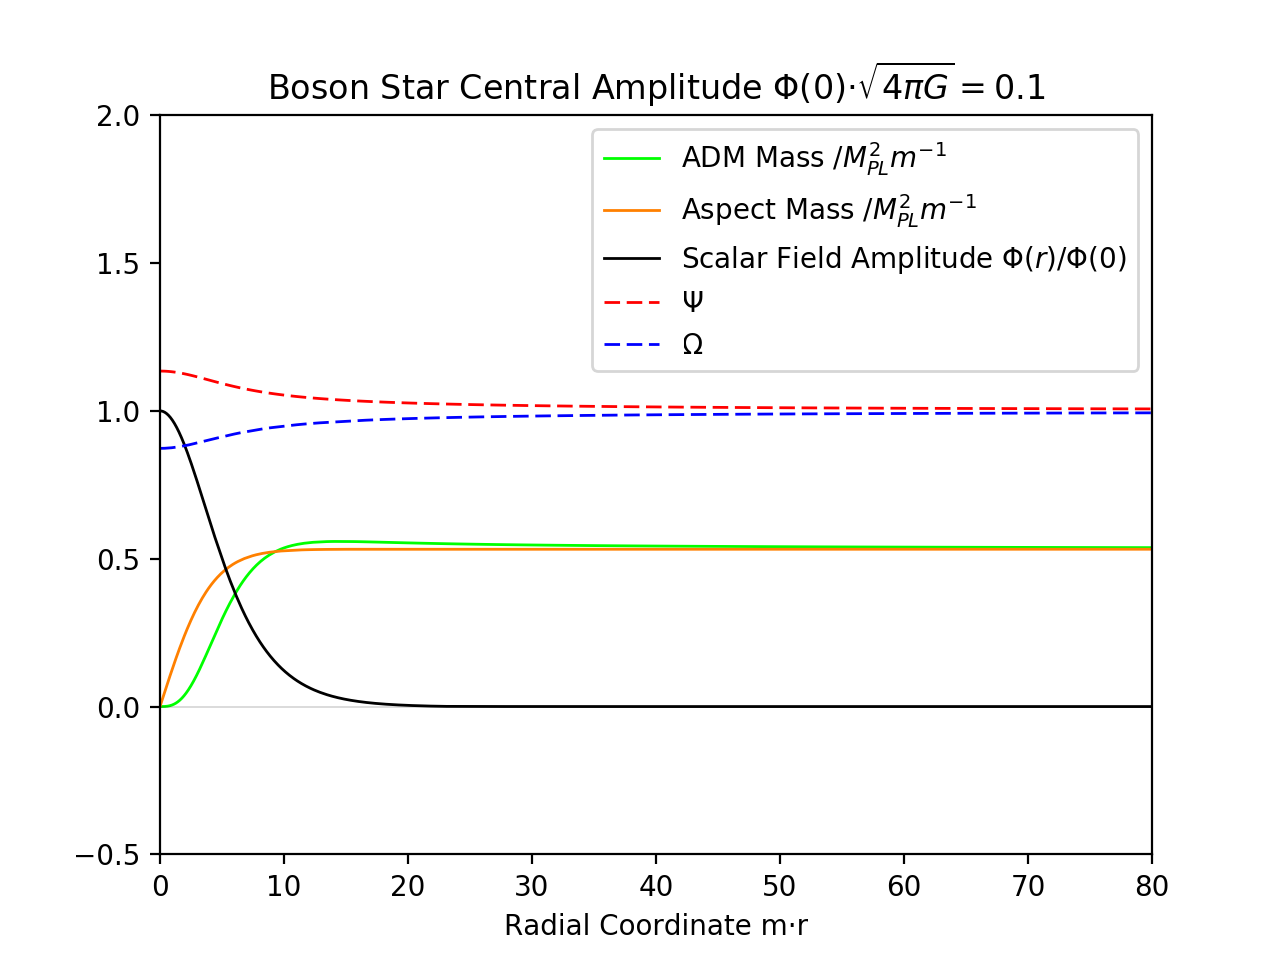
\includegraphics[width=0.8\textwidth]{png/bosonstar_groundstate.png}\label{boson:fig:f1}
\end{figure}

  \begin{figure}[h!]
  \caption{Boson Star radial profile : 1st Excited state}
  \centering
  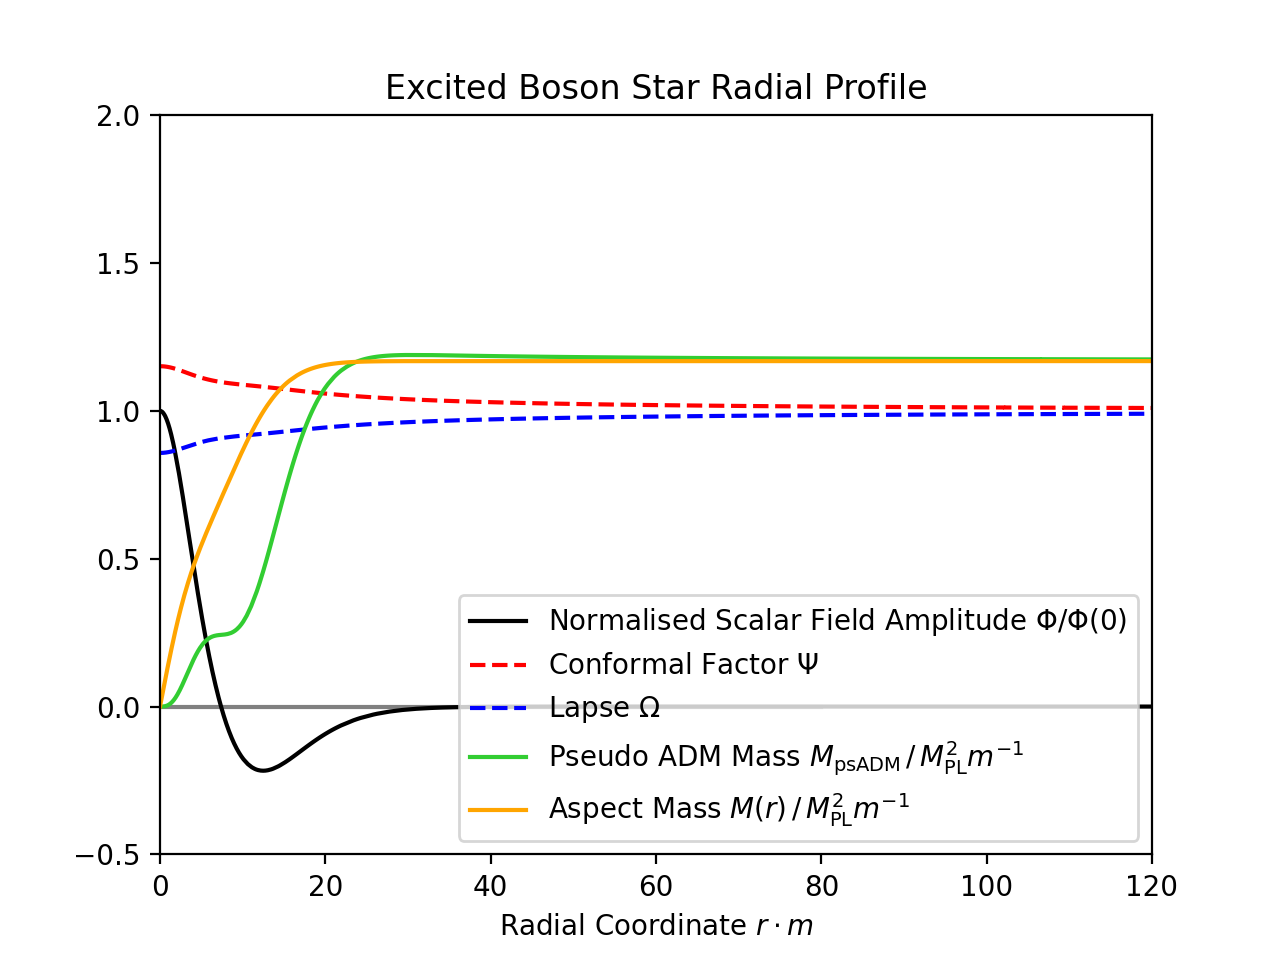
\includegraphics[width=0.8\textwidth]{png/bosonstar_excitedstate.png}\label{boson:fig:f2}
\end{figure}

Figures~\ref{boson:fig:f1} and \ref{boson:fig:f2} show the numerical result for the radial profile of a mini boson star ($\Lambda=0$) and an excited mini boson star. Note two mass definitions are plotted; the ADM mass (calculated as a function of finite r) and the aspect mass $M_A(r)$ which corresponds to assuming the metric's solution is Schwarzschild with $M_A(r)$ rather than $M$. Polytropic fluid stars were also simulated as a preliminary test of the code; they are much easier to create not needing to solve an eigenvalue problem and don't have an asymptotically growing mode. Figures () show how the ADM mass of boson stars varies with central amplitude $\Phi(0)$ and $r_{99}$, the radius which $\Phi(r_{99}) = \Phi(0)/100$. It should be noted that the $\Lambda =0$ case agrees with the known maximum mass, the Kaup limit [] $M_{max} \approx 0.633 {M_{PL}^2}{m^{-1}}$ with the highest measured mass being $ M_{max} = 0.63299(3) {M_{PL}^2}{m^{-1}} $ corresponding to a central amplitude of $\ \sqrt{4\pi G}\Phi(0)_{max} = 0.271(0)$. 

%   \begin{figure}[h!]
%   \caption{Boson star trends, Left: ADM mass vs $\Phi(0)$, Right: ADM mass vs $r_{99}$}
%   \centering
%   \subfloat{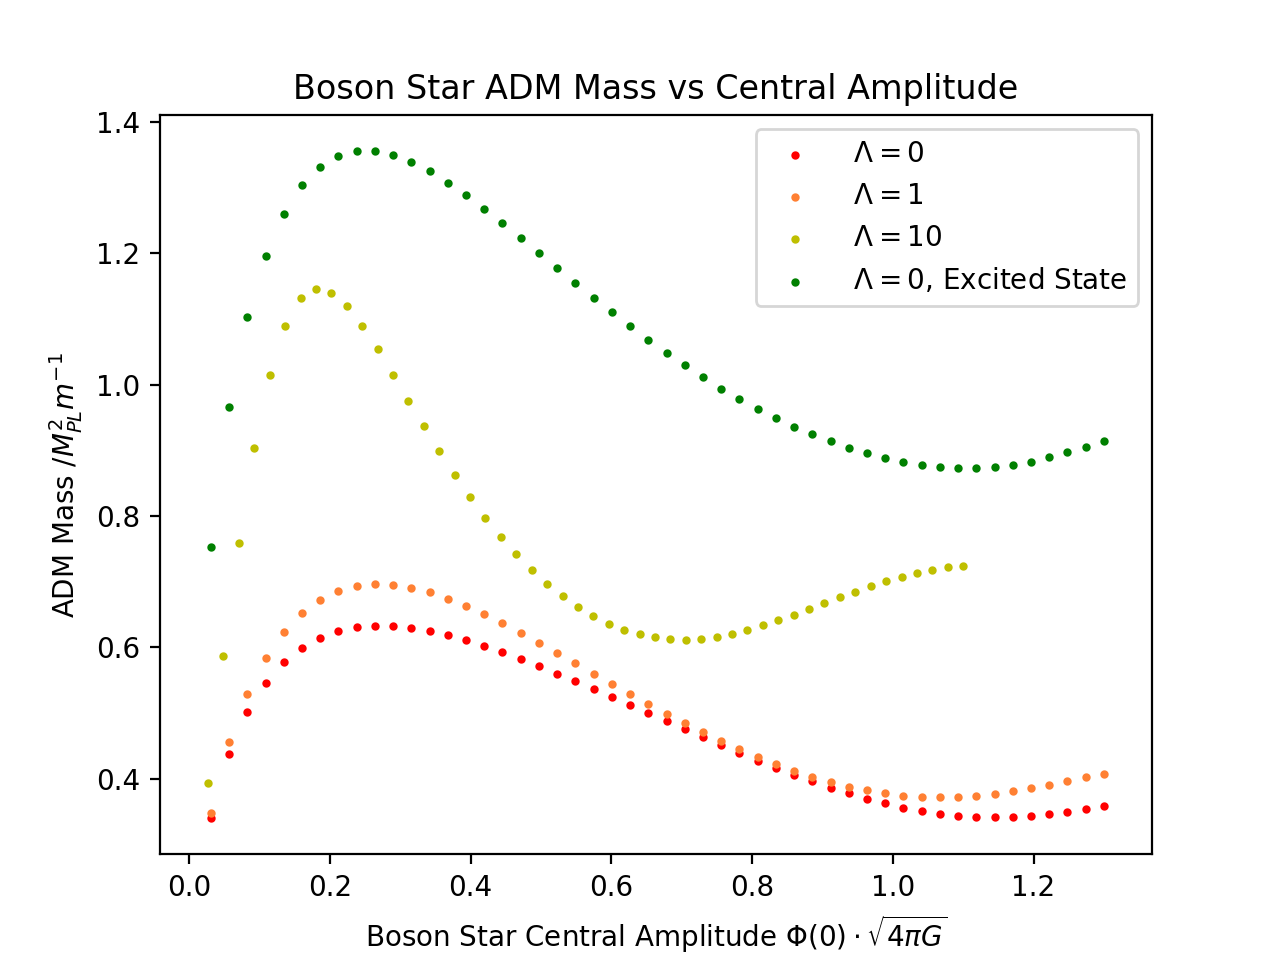
\includegraphics[width=0.5\textwidth]{png/ADM_vs_PC.png}\label{boson:fig:f3}}
%   \hfill
%   \subfloat{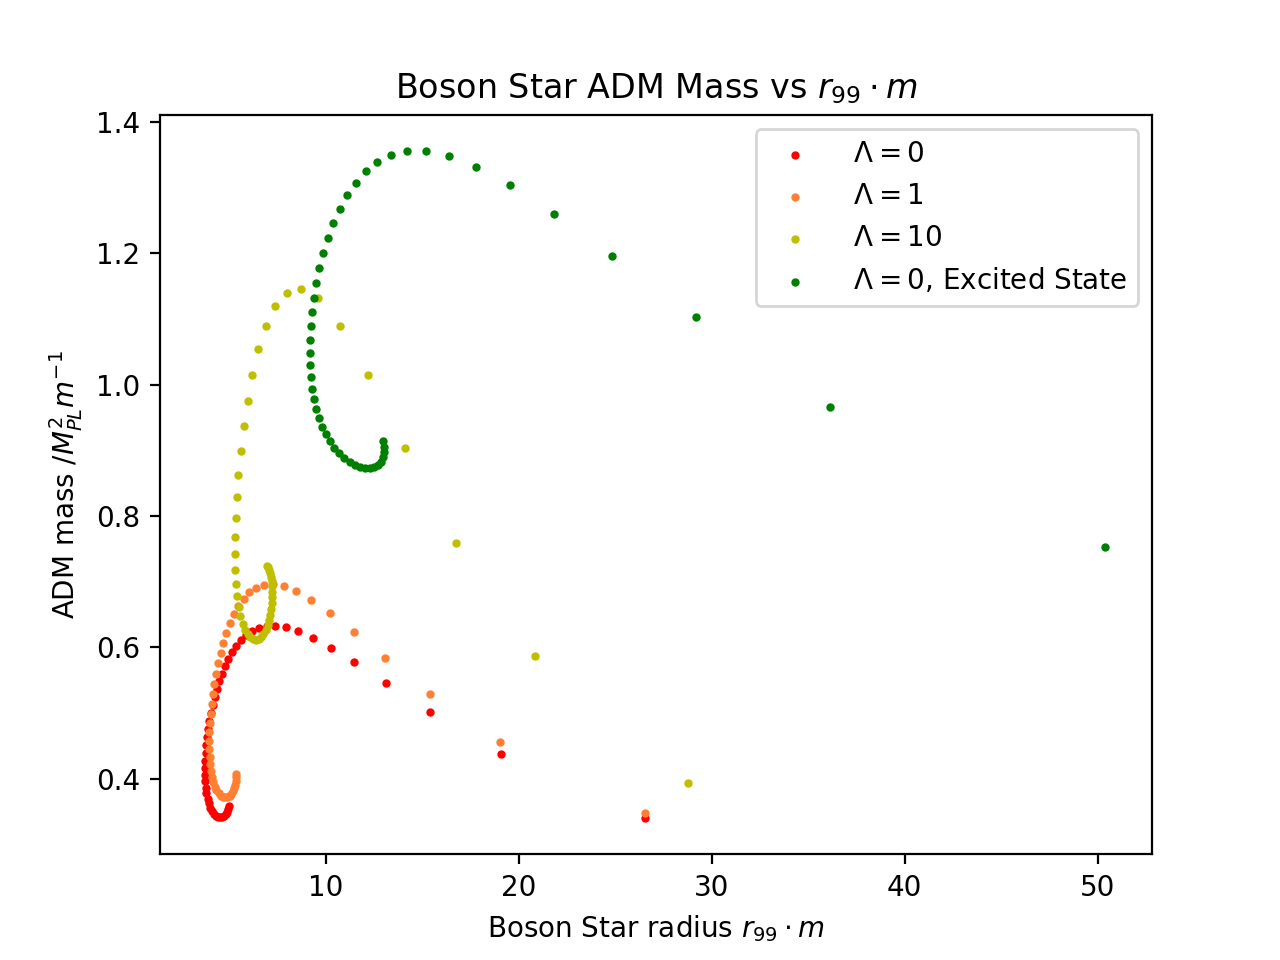
\includegraphics[width=0.5\textwidth]{png/ADM_vs_r99.png}\label{boson:fig:f4}}
% \end{figure}

  \begin{figure}[h!]
  \caption{ADM mass vs $\Phi(0)$}
  \centering
  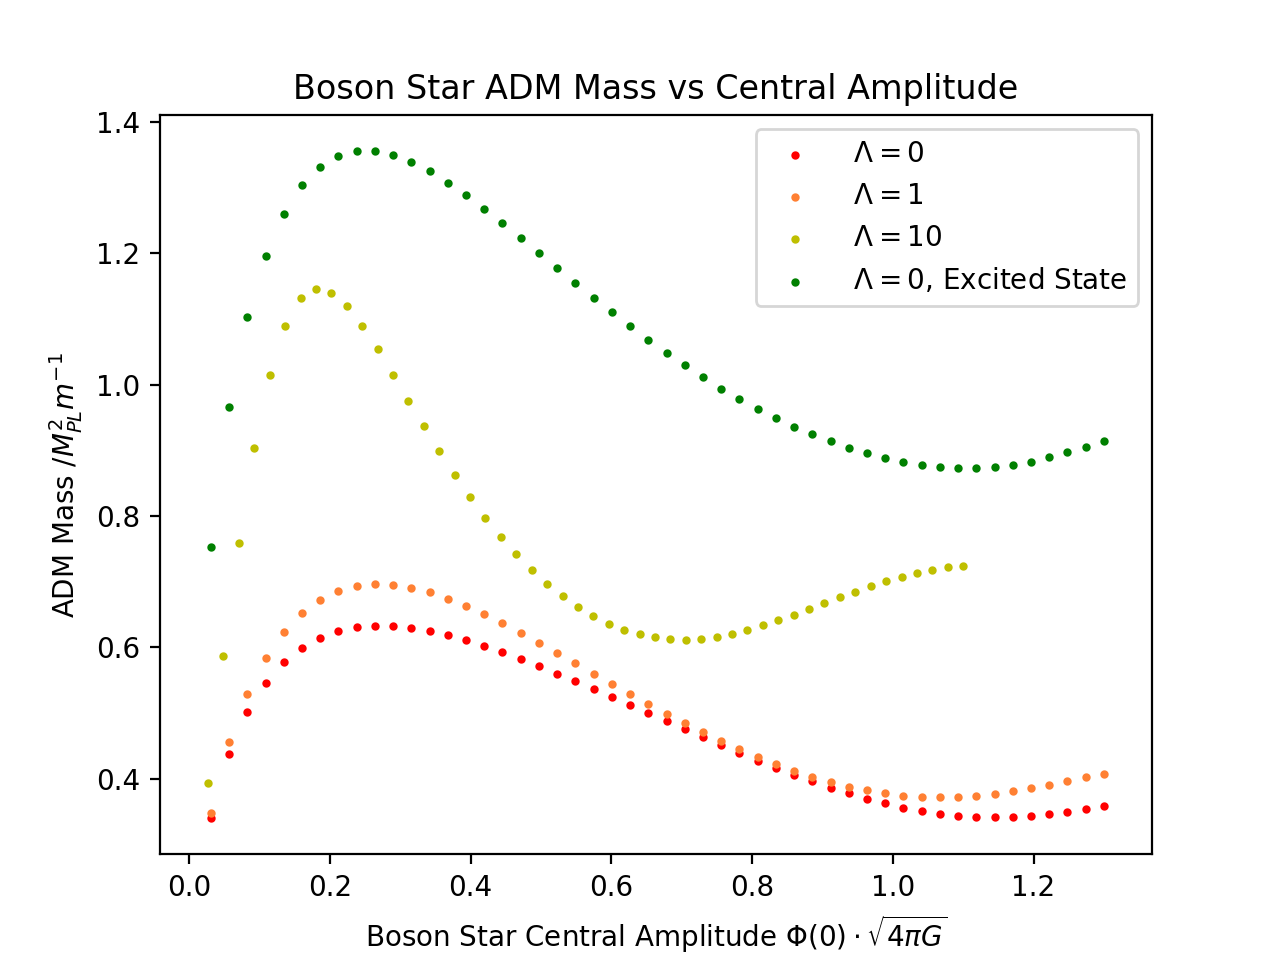
\includegraphics[width=0.8\textwidth]{png/ADM_vs_PC.png}\label{boson:fig:f1}
\end{figure}

  \begin{figure}[h!]
  \caption{ADM mass vs $r_{99}$}
  \centering
  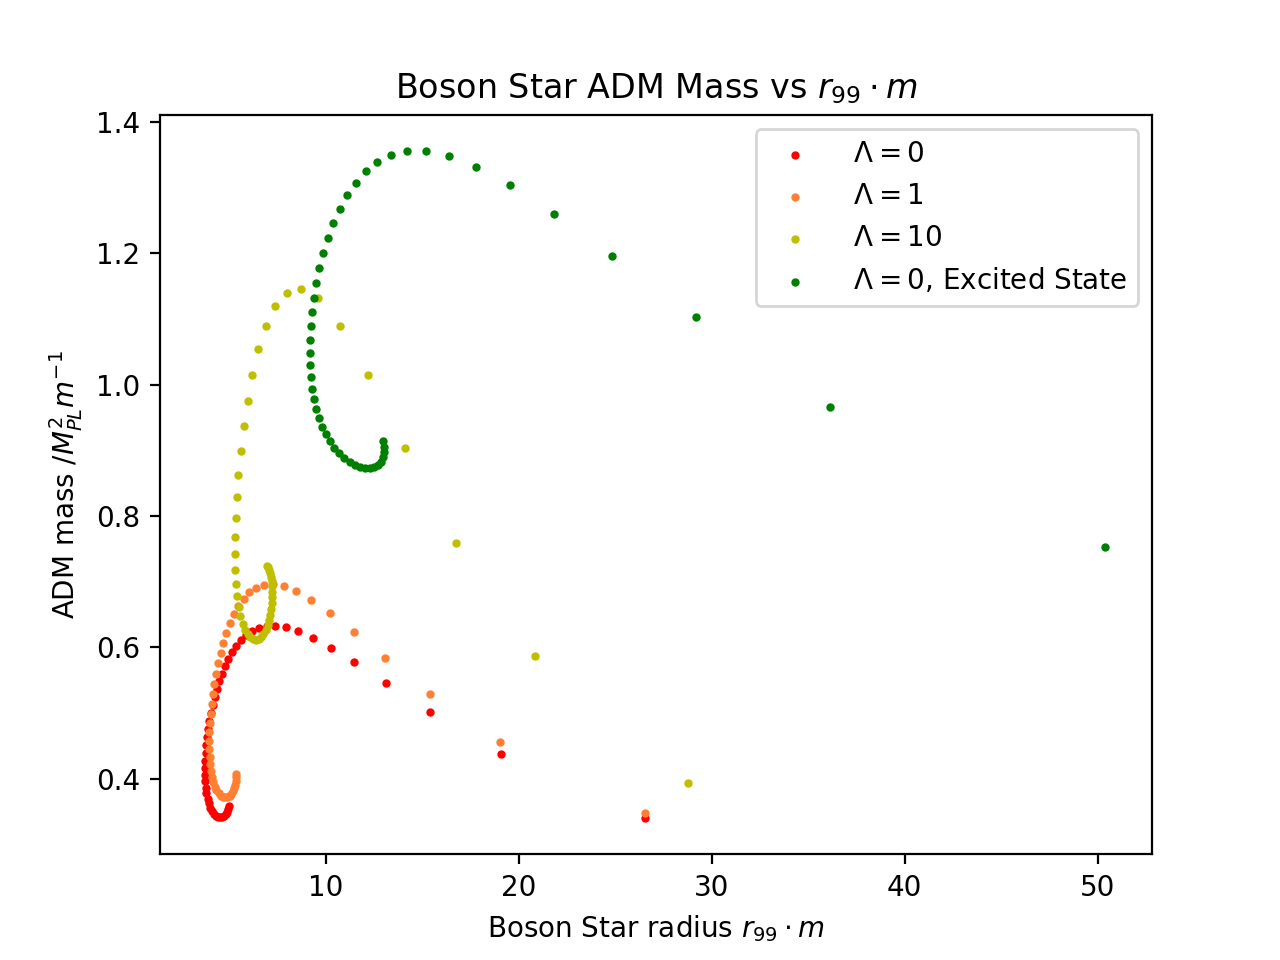
\includegraphics[width=0.8\textwidth]{png/ADM_vs_r99.png}\label{boson:fig:f2}
\end{figure}

While many different boson stars have been made to test the initial data code, all the following evolutions use the same boson star with parameters $\Lambda=0$, $\sqrt{4\pi G}\Phi(0)=0.1 \rightarrow \Phi(0) \approx 0.0282$ and ADM mass $M=0.532(7)$. This is as the stars are heavy enough to form black holes under collisions and large deformations, but stable enough to not collapse to a black hole for moderate perturbations.


EXPLAIN EIGENVALUES AND GROUND STATES BETTER.



\subsection{Single Star Evolutions}
  \begin{figure}[h!]
  \caption{Left: 2D slice of initial $|\vp|$, Right: Maximum of $|\vp|$ during evolution.}
  \centering
  \subfloat{\includegraphics[width=0.5\textwidth]{mod_phi_nice0000.png}\label{boson:fig:f5}}
  \hfill
  \subfloat{\includegraphics[width=0.5\textwidth]{modphimax.png}\label{boson:fig:f6}}
\end{figure}
The first simulation done was of the $\Phi(0)=0.02820$ mini boson star; as mentioned before all simulations are done with this star. The star is supposed to remain in the centre of the grid and not change as it is a rest frame soliton; this is observed through evolution with GRChombo. Figure () shows a rough initial phase in $|\vp|$ which changes significantly upon changing the AMR regridding, hence it is likely only a side effect of the interpolation errors at the boundary of AMR regions. Figure () shows that the star conserves $\mathcal{N}$ upto 4 figures and the constraint $\mathcal{H}$ is driven towards zero as desired.

  \begin{figure}[h!]
  \caption{Left: Total Noether charge $\mathcal{N}$ during evolution, Right: $|| \mathcal{H} ||_2$ during evolution.}
  \centering
  \subfloat{\includegraphics[width=0.5\textwidth]{N.png}\label{boson:fig:f7}}
  \hfill
  \subfloat{\includegraphics[width=0.5\textwidth]{H.png}\label{boson:fig:f8}}
\end{figure}

\subsection{Superposition of Initial Data}
Suppose we have two compact objects with fields $\vp$, $\Pi$, $\gamma_{ij}$, $\K_{ij}$, $\alpha$ and $\beta^i$. The chosen scheme to superpose solutions is below.
\begin{gather*} \vp = \vp^{(1)} + \vp^{(2)}\\
\Pi = \Pi^{(1)} + \Pi^{(2)}\\
 \K^i_j = {\K^{(1)}}^i_j+{\K^{(2)}}^i_j\\
 \gamma_{\mu\nu} = \gamma^{(1)}_{\mu\nu} + \gamma^{(2)}_{\mu\nu}\\
\beta_i = \beta^{(1)}_i + \beta^{(2)}_i \\
 \alpha = \sqrt{\alpha_{(1)}^2 + \alpha_{(2)}^2-1} \quad \mathrm{or}\quad \left[ \alpha_{(1)}^{-1} +  \alpha_{(2)}^{-1}-1\right]^{-1}\\
 \chi = \det{\gamma^{(1)}_{\mu\nu} + \gamma^{(2)}_{\mu\nu}}^{-1/3}\end{gather*}
When a black hole is involved $\Omega(r=\frac{2}{M})=0$ so the event horizon causes the lapse to cross through zero; this is circumvented by setting
\begin{equation} \alpha = \sqrt{\chi}\end{equation}
and the lapse is real, non-negative for a spacelike hypersurface $\Sigma$. Superposing the scalar field $\vp$ is exact for the mini boson star (); for every other variable and type of star case superposition is inexact. Luckily, for sufficiently separated compact objects, superposition gives a very close approximation to the exact numerical solution. The use of CCZ4 also forces the evolution towards a constraint satisfying one. 



\subsection{Head-on Collisions}
All the cases studied here are for stationary initial data $\tilde{\A}_{ij}=0,\K=0$ in-falling from an initial separation of $d \cdot m = 32$ due to gravitational attraction. Firstly we consider the equal mass Boson star binary, initial data in figure (). At first they slowly infall creating a short lived object with three maxima, shown in figure (,left), then collapse to a black hole with a decaying spherical harmonic cloud (figures ) outside. As with all the simulations from now on we assume a black hole forms if $\chi \ll 16^{-1}$ where $\chi=16^-1$ is the value taken on the horizon for the isotropic Schwarzschild metric.
  \begin{figure}[h!]
  \caption{Initial Data, Left: $\chi$, Right: $|\vp|$.}
  \centering
  \subfloat{\includegraphics[width=0.5\textwidth]{headon_bs/chi0000.png}\label{boson:fig:f9}}
  \hfill
  \subfloat{\includegraphics[width=0.5\textwidth]{headon_bs/modphi0000.png}\label{boson:fig:f10}}
\end{figure}
  \begin{figure}[h!]
  \caption{Scalar field amplitude before and after black hole formation, Left: Time $t\cdot m = 150$, Right: Time $t \cdot m = 200$.}
  \centering
  \subfloat{\includegraphics[width=0.5\textwidth]{headon_bs/modphi0003.png}\label{boson:fig:f11}}
  \hfill
  \subfloat{\includegraphics[width=0.5\textwidth]{headon_bs/modphi0004.png}\label{boson:fig:f12}}
\end{figure}
   \begin{figure}[h!]
  \caption{Real part of scalar field after black hole formation, Left: xy plane, Right: yz plane, perpendicular to initial star separation.}
  \centering
  \subfloat{\includegraphics[width=0.5\textwidth]{headon_bs/phi_re0004.png}\label{boson:fig:f13}}
  \hfill
  \subfloat{\includegraphics[width=0.5\textwidth]{headon_bs/phi_re_perp0004.png}\label{boson:fig:f14}}
\end{figure}
 
The second case considered is the same Boson star outside a black hole parameterised by $M=10M_{BS}$ where $M_{BS}$ is the ADM mass of the Boson star. The scalar field tidally deforms into an ellipsoid with high central density, well beyond Kaup limit of $\vp(0)\sim 0.0764$, and spontaneous collapse to a smaller external black hole is observed. After collapse, figure (), there is an elongated cloud about the new small black hole; there are many nodal lines in $\mathrm{Re}(\vp)$ which focus on the large black hole showing the cloud is in-falling.

  \begin{figure}[h!]
  \caption{Initial Data, Left: $\chi$, Right: $|\vp|$.}
  \centering
  \subfloat{\includegraphics[width=0.5\textwidth]{LMR/chi0000.png}\label{boson:fig:f15}}
  \hfill
  \subfloat{\includegraphics[width=0.5\textwidth]{LMR/modphi0000.png}\label{boson:fig:f16}}
\end{figure}
  \begin{figure}[h!]
  \caption{Final Data at time $t\cdot m = 125$, Left: Conformal factor $\chi$, Right: Scalar field modulus $|\vp|$, Bottom: Real part of scalarfield $\mathrm{Re}(\vp).$}
  \centering
  \subfloat{\includegraphics[width=0.5\textwidth]{LMR/chi0005.png}\label{boson:fig:f17}}
  \hfill
  \subfloat{\includegraphics[width=0.5\textwidth]{LMR/modphi0005.png}\label{boson:fig:f18}}
  \\
   \subfloat{\includegraphics[width=0.5\textwidth]{LMR/phi_re0000.png}\label{boson:fig:f19}}
\end{figure}
Final case consists of an equal mass Black Hole and Boson Star, initial configuration in Figure 11. As can be seen from the plot of $\Re(\phi)$ and $|\phi|$, in Figure 12, most of the star falls into the black hole, however some scalar field manages to excite an intricate spherical harmonic cloud pattern.
  \begin{figure}[h!]
  \caption{Initial data for equal mass Boson Star and Black Hole, Left: $\chi$, Right: $|\vp|$}
  \centering
  \subfloat{\includegraphics[width=0.5\textwidth]{headon/chi0000.png}\label{boson:fig:f20}}
  \hfill
  \subfloat{\includegraphics[width=0.5\textwidth]{headon/mod_phi0000.png}\label{boson:fig:f21}}
\end{figure}
  \begin{figure}[h!]
  \caption{Time $t\cdot m=905$ for equal mass Boson Star and Black Hole, Left: $\Re(\vp)$, Right: $|\vp|$}
  \centering
  \subfloat{\includegraphics[width=0.5\textwidth]{headon/phi_re0000.png}\label{boson:fig:f22}}
  \hfill
  \subfloat{\includegraphics[width=0.5\textwidth]{headon/mod_phi0007.png}\label{boson:fig:f23}}
\end{figure}

In all three cases, the Noether charge drops rapidly upon the formation of a black hole; this will be explained in the next section. However some scalar field lingers after collapse, in each case the hair takes the form of spherical harmonics discussed in (). Also observed is the decay of the spherical harmonics to zero amplitude in these simulations with no angular momentum. 
 
\subsection{Binary Inspiral}
The only considered case here is the Quasi-circular orbit and inspiral of two equal mass boson stars. The initial boosts were determined by a newtonian calculation yielding 
\begin{equation} v^2 = \frac{M}{2d}\end{equation}
where $M=0.53(29)$ is the ADM mass of the Boson Star and d is the initial separation. For a relatively low separation of $d\cdot m =32$ code units, shown in Figures 13,14 (Left), we get $v \sim 0.0915$. The boson stars are observed to complete roughly half an orbit before merging and collapse, forming a black hole. Here a Kerr black hole is assumed to have formed as the spacetime has a significant angular momentum which should partially infall with the scalar field. 

  \begin{figure}[h!]
  \caption{Boson Star $|\vp|$. Left: initial data, Right: later time $t \cdot m = 700$}
  \centering
  \subfloat{\includegraphics[width=0.5\textwidth]{inspiral/mod_phi_inspiral_nice0000.png}\label{boson:fig:f24}}
  \hfill
  \subfloat{\includegraphics[width=0.5\textwidth]{inspiral/mod_phi_inspiral_nice0002.png}\label{boson:fig:f25}}
\end{figure}
  \begin{figure}[h!]
  \caption{Boson Star $\Re(\vp)$. Left: initial data, Right: later time $t \cdot m = 700$}
  \centering
  \subfloat{\includegraphics[width=0.5\textwidth]{inspiral/phi_inspiral_nice0000.png}\label{boson:fig:f26}}
  \hfill
  \subfloat{\includegraphics[width=0.5\textwidth]{inspiral/phi_inspiral_nice0002.png}\label{boson:fig:f27}}
\end{figure}
  \begin{figure}[h!]
  \caption{Left: Total Noether charge $\mathcal{N}$ during evolution, Right: $\Psi_4$ over 22 harmonic during evolution.}
  \centering
  \subfloat{\includegraphics[width=0.5\textwidth]{inspiral/N.png}\label{boson:fig:f28}}
  \hfill
  \subfloat{\includegraphics[width=0.5\textwidth]{inspiral/GW.png}\label{boson:fig:f29}}
\end{figure}
Figure 15 shows the total Noether charge, which is no longer conserved. When the black hole forms, the in-falling scalar field moves towards zero radius and gets hugely compressed. The huge compression causes extreme field gradients which induces continuous regridding in the AMR, but this is capped at 7 layers in this simulation to make runtime feasible. When the 8th AMR level is needed it is simply not added and resolution becomes low enough that any Noether charge near the centre is so under-resolved that it seems to fall between the gridpoints. Interestingly, Figures 13,14 (Right) show a scalar field configuration lingering around the black hole, mostly outside the contour $\chi=0.7$, looking like scalar hair. Also Figure 15 (Left) of the Noether charge appears to take significantly longer to decay than in the linear collision simulations. It can be seen in Figure 14 in the plot of $\Re(\vp)$ that the cloud has angular nodes corresponding to angular momentum similarly to boosted stars picking up nodal planes perpendicular to momentum and Figure 10 (Bottom) of the infalling cloud. 

The gravitational wave (GW) signal can be seen in Figure 15 (Right), extracted at a radius $r \cdot m = 90$. At the time $t \cdot m \approx 700$ the gravitational wave signal due to the merger appears; in order to record a longer inspiral simulations with larger initial separations need to be simulated. Currently there appears to be some small problem with the initial data, also observed in the collisions with no angular momentum, that manifests itself in noisy GW extraction and the Hamiltonian constraint initially sharply rising. 

  \subsection{STUFF}
  I think I want a stationary star
  headon collision
  maybe collison with angular momentum
  collision of bs with bh